\documentclass{article}
\usepackage{a4wide}
\usepackage[T1]{fontenc}
\usepackage[utf8]{inputenc}
\usepackage[french]{babel}
\usepackage{empheq}
\usepackage{mathtools, bm}
\usepackage{amssymb, bm}
\usepackage{graphicx}
\usepackage{caption}
\usepackage{subcaption}
\usepackage{hyperref}
\usepackage{csvsimple}
\usepackage{float}

\title{\textbf{\Huge  Université Paris Saclay}\\ Rapport IAS}
\author{Guillaume Abadie, Jérôme Coquisart, Mathis Dupon, Martin Vitani}
\date{Année 2021}


\begin{document}
    \maketitle
    \tableofcontents
    \newpage


    \section{Introduction au problème}
    La ville de Chicago a un ratio de crimes, surtout sur les crimes violents, au dessus de la moyenne
    nationale des États-Unis.
    Les crimes dans le ville on été collectés dès le début du 20ème siècle pour essayer de 
    comprendre pourquoi la ville était sujette à autant de violence.
    Le dataset correspond aux crimes commis entre 2001 et 2020.
    Tous les jours, la police de Chicago alimente la base de donnée avec les nouveaux crimes commis
    dans la ville. Seuls les meurtres ne sont pas comptabilisé dans notre dataset.

    \section{Aperçu du dataset}
    \begin{figure}[H]
            \centering
	    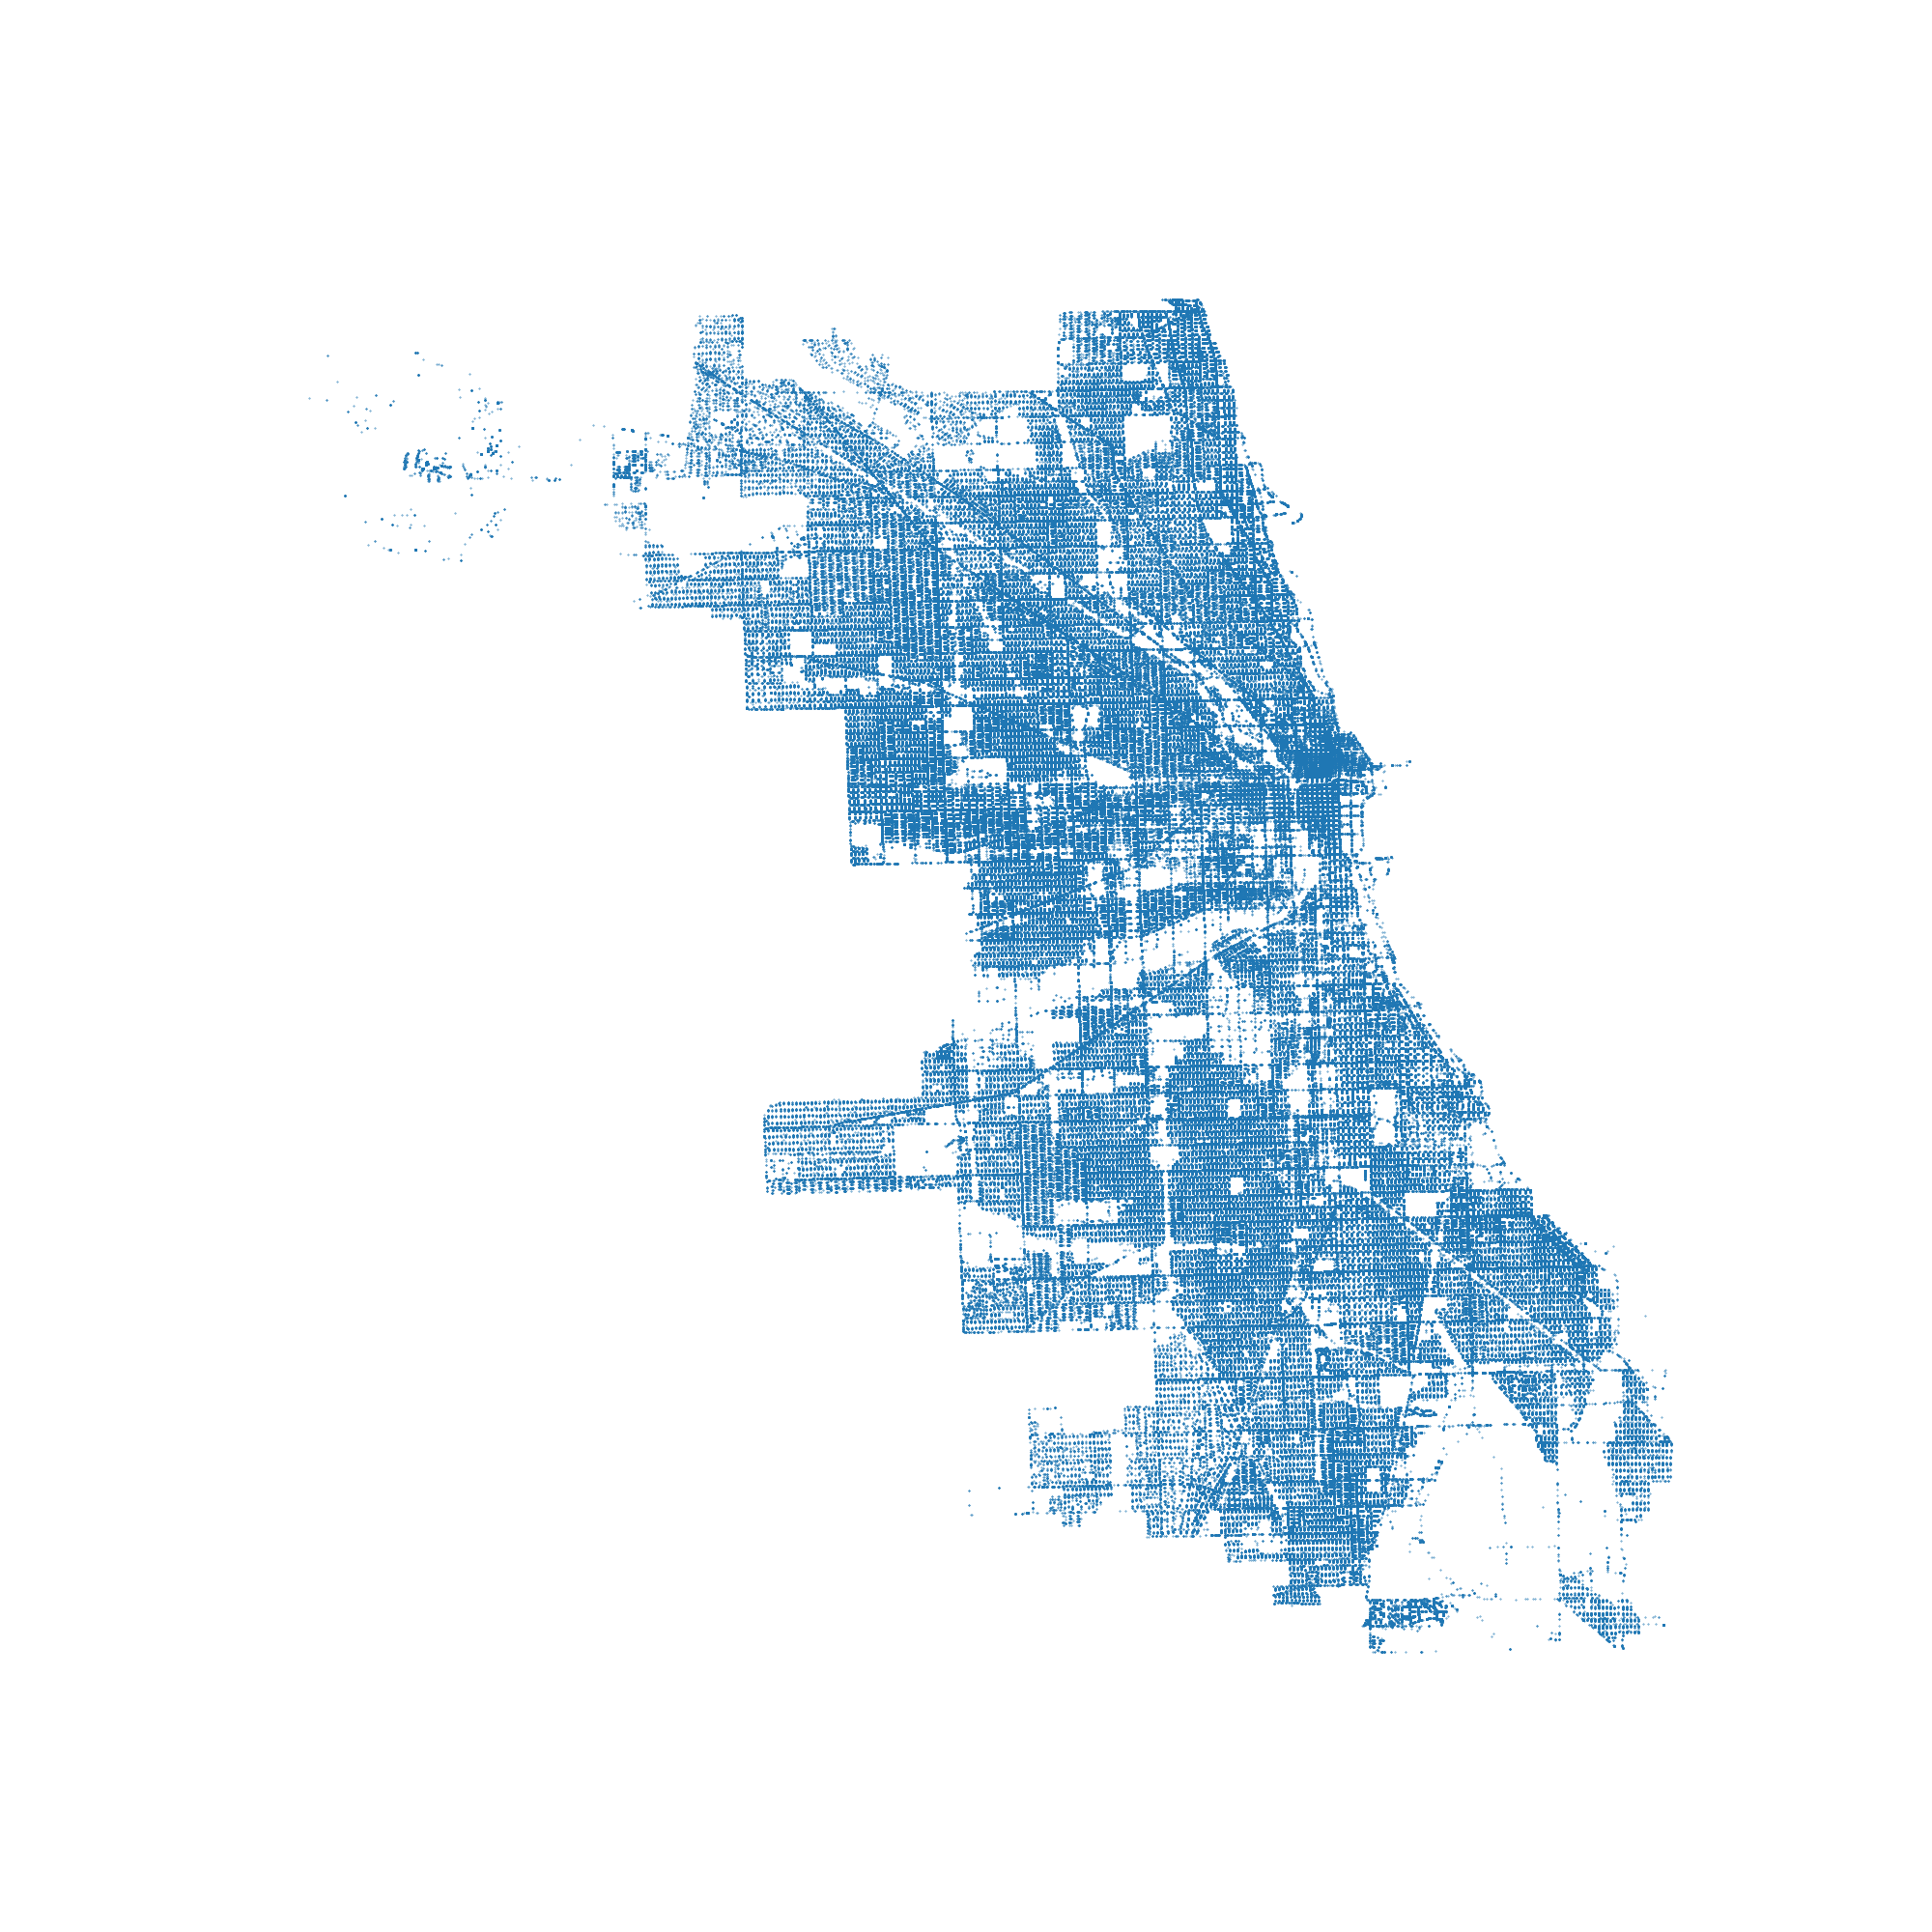
\includegraphics[scale=.2]{carte_chicago.png}
    \end{figure}

    \section{Définition du problème}

    \section{Préprocessing}
    \begin{figure}[H]
            \centering
	    \includegraphics[scale=.2]{carte_densité.png}
    \end{figure}

    \section{Choix d'algorithme}

    \section{Comparaison des modèles}

    \section{Présentation des résultats}

    \section{Conclusion}

\end{document}
